\documentclass[border=6pt]{standalone}
\usepackage{tikz}
\usetikzlibrary{arrows.meta}
\begin{document}
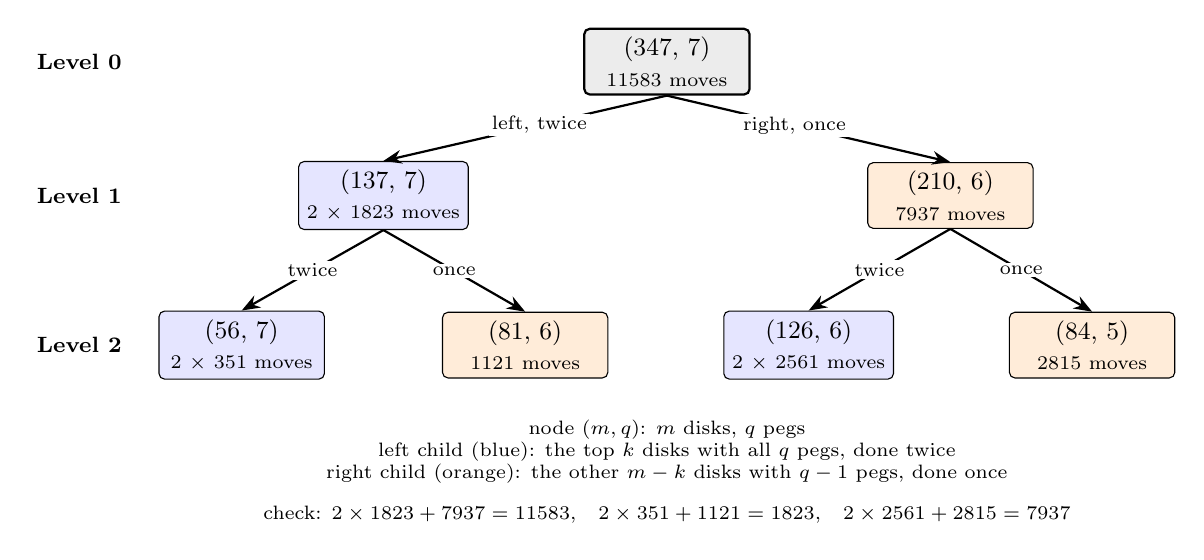
\begin{tikzpicture}[>=Stealth,font=\small,
 n/.style={draw,rounded corners=2pt,align=center,minimum width=2.1cm,inner sep=3pt},
 root/.style={n,thick,fill=gray!15},
 lft/.style={n,fill=blue!10},
 rgt/.style={n,fill=orange!15},
 e/.style={->,thick},
 lab/.style={font=\scriptsize,fill=white,inner sep=1pt}]
\node[root] (r) at (0,0) {$(347,\,7)$\\{\scriptsize 11583 moves}};
\node[lft] (a) at (-3.6,-1.7) {$(137,\,7)$\\{\scriptsize 2 $\times$ 1823 moves}};
\node[rgt] (b) at (3.6,-1.7) {$(210,\,6)$\\{\scriptsize 7937 moves}};
\node[lft] (aa) at (-5.4,-3.6) {$(56,\,7)$\\{\scriptsize 2 $\times$ 351 moves}};
\node[rgt] (ab) at (-1.8,-3.6) {$(81,\,6)$\\{\scriptsize 1121 moves}};
\node[lft] (ba) at (1.8,-3.6) {$(126,\,6)$\\{\scriptsize 2 $\times$ 2561 moves}};
\node[rgt] (bb) at (5.4,-3.6) {$(84,\,5)$\\{\scriptsize 2815 moves}};
\draw[e] (r.south) -- node[lab,pos=0.45]{left, twice} (a.north);
\draw[e] (r.south) -- node[lab,pos=0.45]{right, once} (b.north);
\draw[e] (a.south) -- node[lab]{twice} (aa.north);
\draw[e] (a.south) -- node[lab]{once} (ab.north);
\draw[e] (b.south) -- node[lab]{twice} (ba.north);
\draw[e] (b.south) -- node[lab]{once} (bb.north);
\foreach \y/\t in {0/Level 0,-1.7/Level 1,-3.6/Level 2} \node[font=\footnotesize\bfseries,anchor=east] at (-6.8,\y) {\t};
\node[font=\scriptsize,align=center] at (0,-4.95) {node $(m,q)$: $m$ disks, $q$ pegs\\left child (blue): the top $k$ disks with all $q$ pegs, done twice\\right child (orange): the other $m-k$ disks with $q-1$ pegs, done once};
\node[font=\scriptsize] at (0,-5.75) {check: $2\times1823+7937=11583$,\quad $2\times351+1121=1823$,\quad $2\times2561+2815=7937$};
\end{tikzpicture}
\end{document}
